\documentclass[a4paper, man, floatsintext]{apa6}
\usepackage{lmodern}
\usepackage{amssymb,amsmath}
\usepackage{ifxetex,ifluatex}
\usepackage{fixltx2e} % provides \textsubscript
\ifnum 0\ifxetex 1\fi\ifluatex 1\fi=0 % if pdftex
  \usepackage[T1]{fontenc}
  \usepackage[utf8]{inputenc}
\else % if luatex or xelatex
  \ifxetex
    \usepackage{mathspec}
  \else
    \usepackage{fontspec}
  \fi
  \defaultfontfeatures{Ligatures=TeX,Scale=MatchLowercase}
\fi
% use upquote if available, for straight quotes in verbatim environments
\IfFileExists{upquote.sty}{\usepackage{upquote}}{}
% use microtype if available
\IfFileExists{microtype.sty}{%
\usepackage{microtype}
\UseMicrotypeSet[protrusion]{basicmath} % disable protrusion for tt fonts
}{}
\usepackage{hyperref}
\hypersetup{unicode=true,
            pdfauthor={Jana B. Jarecki},
            pdfborder={0 0 0},
            breaklinks=true}
\urlstyle{same}  % don't use monospace font for urls
\usepackage{graphicx,grffile}
\makeatletter
\def\maxwidth{\ifdim\Gin@nat@width>\linewidth\linewidth\else\Gin@nat@width\fi}
\def\maxheight{\ifdim\Gin@nat@height>\textheight\textheight\else\Gin@nat@height\fi}
\makeatother
% Scale images if necessary, so that they will not overflow the page
% margins by default, and it is still possible to overwrite the defaults
% using explicit options in \includegraphics[width, height, ...]{}
\setkeys{Gin}{width=\maxwidth,height=\maxheight,keepaspectratio}
\IfFileExists{parskip.sty}{%
\usepackage{parskip}
}{% else
\setlength{\parindent}{0pt}
\setlength{\parskip}{6pt plus 2pt minus 1pt}
}
\setlength{\emergencystretch}{3em}  % prevent overfull lines
\providecommand{\tightlist}{%
  \setlength{\itemsep}{0pt}\setlength{\parskip}{0pt}}
\setcounter{secnumdepth}{0}
% Redefines (sub)paragraphs to behave more like sections
\ifx\paragraph\undefined\else
\let\oldparagraph\paragraph
\renewcommand{\paragraph}[1]{\oldparagraph{#1}\mbox{}}
\fi
\ifx\subparagraph\undefined\else
\let\oldsubparagraph\subparagraph
\renewcommand{\subparagraph}[1]{\oldsubparagraph{#1}\mbox{}}
\fi

%%% Use protect on footnotes to avoid problems with footnotes in titles
\let\rmarkdownfootnote\footnote%
\def\footnote{\protect\rmarkdownfootnote}

%%% Change title format to be more compact
\usepackage{titling}

% Create subtitle command for use in maketitle
\providecommand{\subtitle}[1]{
  \posttitle{
    \begin{center}\large#1\end{center}
    }
}

\setlength{\droptitle}{-2em}

  \title{}
    \pretitle{\vspace{\droptitle}}
  \posttitle{}
    \author{Jana B. Jarecki}
    \preauthor{\centering\large\emph}
  \postauthor{\par}
      \predate{\centering\large\emph}
  \postdate{\par}
    \date{16 September, 2019}

\usepackage{natbib} \usepackage{threeparttable} \usepackage{booktabs}
\shorttitle{test} \usepackage{setspace}
\AtBeginEnvironment{tabular}{\singlespacing} \usepackage{times}
\usepackage{changes} \usepackage{upgreek}
\AtBeginDocument{\let\maketitle\relax}

\begin{document}

\subsection{Evaluations of Gambles by Condition and Sample Size}

Table \ref{tab:meansStudy1} shows participants' evaluations of the
gambles in the experience and description conditions. The evaluations in
the experience condition are not a linear function of sample size. In
the best mixed regression model \(\mathrm{M}\textsubscript{0}\) gamble
type (p-bet vs. \$-bet) has a (fixed) effect on evaluations and sample
size is only a random factor. It outperforms a model with sample size as
fixed effect (\(BF\textsubscript{01} = 409\)) and a model with
sample-size\(\times\)gamble-type interaction
(\(BF\textsubscript{01} > 1,000\)).

\begin{figure}

{\centering 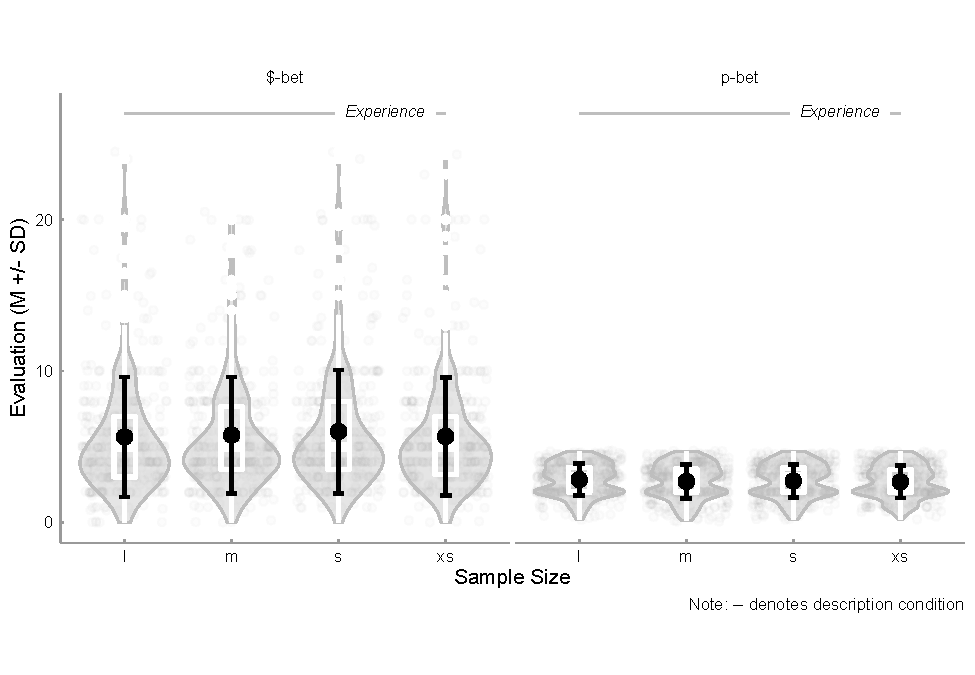
\includegraphics{../figures/study1_evaluations-1} 

}

\caption{Mean gamble evaluations of \$-bets and p-bets in the experience condition across sample sizes and in the the description condition.}\label{fig:study1_evaluations}
\end{figure}

\begin{table}[tbp]
\begin{center}
\begin{threeparttable}
\caption{\label{tab:meansStudy1}Valuations of Gambles in Study 1}
\begin{tabular}{lcccrr}
\toprule
Condition & Sample size & \textit{Med} & \textit{M} & D--E & D--E:$BF\textsubscript{10}$\\
\midrule
Gamble ID 1 &  &  &  &  & \\
\ \ \ E & xs & 5.00 & 5.21 & -0.71 & 4.28\\
\ \ \ E & s & 5.00 & 5.41 & -0.91 & 99.96\\
\ \ \ E & m & 5.00 & 5.51 & -1.01 & 75.80\\
\ \ \ E & l & 5.00 & 5.44 & -0.94 & 1,952.17\\
\ \ \ D & -- & 4.00 & 4.50 & NA & NA\\
Gamble ID 2 &  &  &  &  & \\
\ \ \ E & xs & 4.00 & 4.38 & -0.63 & 11.38\\
\ \ \ E & s & 4.00 & 4.40 & -0.66 & 45.62\\
\ \ \ E & m & 4.00 & 4.17 & -0.43 & 1.23\\
\ \ \ E & l & 4.00 & 4.02 & -0.27 & 0.48\\
\ \ \ D & -- & 3.40 & 3.75 & NA & NA\\
Gamble ID 3 &  &  &  &  & \\
\ \ \ E & xs & 6.00 & 7.46 & -0.27 & 0.39\\
\ \ \ E & s & 6.95 & 8.47 & -1.28 & 9.64\\
\ \ \ E & m & 6.65 & 8.05 & -0.86 & 6.47\\
\ \ \ E & l & 6.00 & 8.04 & -0.85 & 1.13\\
\ \ \ D & -- & 5.60 & 7.19 & NA & NA\\
Gamble ID 4 &  &  &  &  & \\
\ \ \ E & xs & 3.00 & 2.81 & 0.32 & 58,898.63\\
\ \ \ E & s & 3.20 & 3.01 & 0.12 & 0.55\\
\ \ \ E & m & 3.00 & 2.85 & 0.28 & 30.36\\
\ \ \ E & l & 3.20 & 3.00 & 0.13 & 1.43\\
\ \ \ D & -- & 3.20 & 3.13 & NA & NA\\
Gamble ID 5 &  &  &  &  & \\
\ \ \ E & xs & 2.00 & 1.79 & 0.11 & 2.99\\
\ \ \ E & s & 2.00 & 1.79 & 0.11 & 3.18\\
\ \ \ E & m & 2.00 & 1.78 & 0.12 & 6.78\\
\ \ \ E & l & 2.00 & 1.85 & 0.05 & 0.35\\
\ \ \ D & -- & 2.00 & 1.90 & NA & NA\\
Gamble ID 6 &  &  &  &  & \\
\ \ \ E & xs & 4.00 & 3.51 & 0.09 & 0.48\\
\ \ \ E & s & 4.00 & 3.57 & 0.02 & 0.28\\
\ \ \ E & m & 4.00 & 3.64 & -0.04 & 0.16\\
\ \ \ E & l & 4.00 & 3.70 & -0.10 & 0.33\\
\ \ \ D & -- & 4.00 & 3.60 & NA & NA\\
\bottomrule
\addlinespace
\end{tabular}
\begin{tablenotes}[para]
\normalsize{\textit{Note.} \textit{M} = mean, \textit{Med} = median, D--E = difference between mean description-based valuations and experience-based valuations, $BF\textsubscript{10}$ = Bayes Factor quantifying the evidence for a linear model $\mathrm{M}\textsubscript{1}$ predicting that valuations differ between description and experience over a linear model $\mathrm{M}\textsubscript{0}$ predicting no such differences; both models models contain a by-participant random effect. Gambles IDs 1, 2, and 3 are \$-bets; Gamble IDs 4, 5, and 6 are p-bets.}
\end{tablenotes}
\end{threeparttable}
\end{center}
\end{table}

\subsection{Cognitive Modeling of Evaluations by Sample Size}

To examine the role of sample size in value judgments more closely, we
used cognitive computational modeling. We compared the performance of
the \added{relative frequency} (RF) model and the
\added{Bayesian value updating} (BVU) model regarding the observed
evaluations.
\added{The models were compared to a baseline model, predicting a constant evaluation equal to the mean  individual evaluation (sensible models are expected to outperform this baseline model).}

\subsubsection{Modeling Procedure} 
\added{The observed and predicted evaluations were normalized to a common range (0 - 1, by division through the gain magnitude and truncation of normalized values $>$ 1). The free model parameters were estimated by maximum likelihood at the participant level, assuming observations follow a truncated normal distribution (truncation: 0-1) around the model predictions with a constant standard deviation ($\sigma$) estimated as a free parameter ($0 < \sigma \leq 1$).  Therefore, the RF model had 2 free parameter, the power utility exponent $\alpha$ ($0 \leq \alpha \leq 20$) and $\sigma$. The BVU model had 4 free parameter the gain prior $\theta_G$ ($0 \leq \theta_G \leq 1$; the loss prior was $\theta_0=2-\theta_G$), the learning rate $\delta$ ($0 \leq \delta \leq 10$), $\alpha$ and $\sigma$. A 3-parameter BVU model was also tested, constraining the BVU to have a fixed learning rate of $\delta=1$ (optimal Bayesian updating). The baseline model had 2 free parameter, the mean evaluation $\mu$ and $\sigma$. Parameters were estimated by a local nonlinear optimization solver solnp using the R package solnp (REF). The model comparison used the Bayesian information criterion (BIC), transformed into Bayesian evidence weights (\citealp{Kass1995, Lewandowsky2011}).}

\subsubsection{Modeling Results}

The Bayesian value updating model described most participants best (23
of 33; 70\%), and the relative frequency model described a minority of
participants (8; 24\%). The baseline model described 2 participants
best. The 3-parameter Bayesian value updating model (BVU \(\delta=1\))
described no participant best. Figure \ref{fig:model_weights} shows the
evidence strength for the models by participant. It becomes evident that
the 3-parameter BVU competes mostly with the full BVU model. The median
(across participant) Bayesian information criterion (BIC) of the models
was BIC\textsubscript{BVU}\(=\) 66.4 BIC\textsubscript{BCU $\delta=1$}
\(=\) 61.7, BIC\textsubscript{RF}\(=\) 61.1.

\begin{figure}

{\centering 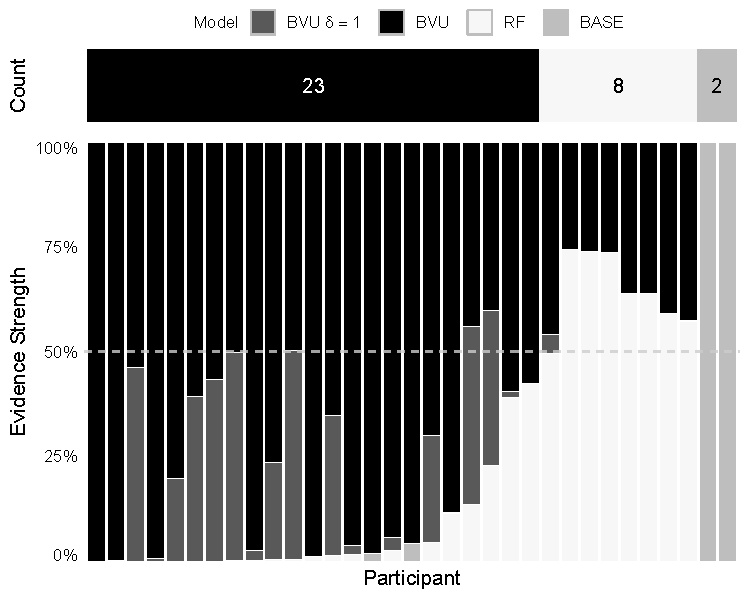
\includegraphics{../figures/model_weights-1} 

}

\caption{Evidence for the models for individual participants. RF: relative frequency model, BVU: Bayesian value updating model, BASE: Baseline model.}\label{fig:model_weights}
\end{figure}

The estimated parameter of the winning models
(Table\textasciitilde{}\ref{tab:model_par}) reveal no apparent
difference between the utility (power utility exponent \(\alpha\))
between those participants using the Bayesian value updating
(\(M=1.68\)) and those using a relative frequency strategy (\(M=1.73\))
\(\Delta M = -0.05\), 95\% CI \([-0.78\), \(0.67]\),
\(t(29.00) = -0.15\), \(p = .883\). The resulting parameters of the
Bayesian model also indicate a prior belief in zero outcomes being more
likely (62\%) than a gain (\(\theta_G = 0.77, \theta_0 = 1.23\) prior on
gains and zeros, respectively). Interestingly, the estimated learning
rate (\(\delta\)) was anti-conservative (values \(<\) 1 mean
conservative, 1 is optimal Bayesian, \(>\) 1 is liberal learning),
unlike usually conservative Bayesian learners
\citep{Edwards1967,Tauber2017}).

\begin{table}[tbp]
\begin{center}
\begin{threeparttable}
\caption{\label{tab:model_par}Parameter Estimates of Winning Models (\textit{M (SD)})}
\begin{tabular}{lccccc}
\toprule
Winning Model & $\alpha$ & $\delta$ & $\theta_G$ & $\mu$ & $\sigma$\\
\midrule
BVU (\textit{n}$=$23) & 1.68 (1.48) & 1.53 (2.27) & 0.77 (0.58) & - & 0.12 (0.07)\\
RF (\textit{n}$=$8) & 1.73 (0.49) & - & - & - & 0.12 (0.02)\\
BASE (\textit{n}$=$2) & - & - & - & 0.48 (0.01) & 0.22 (0.10)\\
\bottomrule
\addlinespace
\end{tabular}
\begin{tablenotes}[para]
\normalsize{\textit{Note.} BVU: Bayesian value updating model, RF: relative frequency model, BASE: baseline model. Parameters denote: $\alpha=$ power utility exponent, $\delta=$ learning rate, $\theta_G$ gain prior, $\mu=$ mean evaluation, $\sigma$ standard deviation.}
\end{tablenotes}
\end{threeparttable}
\end{center}
\end{table}


\end{document}
